\section{Sammensetning}
\label{sec:sammensetning}
Ved oppstart ble studentene involvert i EiT-landsbyen delt inn i grupper. Disse gruppene var fordelt slik at de skulle oppnå en størst mulig tverrfaglighet. Under vil en presentasjon av hvert enkelt medlem av gruppen bli gitt i tillegg til en uttalelse fra personen om forventninger og ambisjoner i faget.
Espen er en 22 år gammel gutt fra Tromsø. Han karakterisere seg selv som utadvent, ærlig og detaljeorientert, men kan være sta i noen tilfeller. På fritiden går mye av tiden til sport, teknologi, film og musikk, samt reiser. Den faglige bakgrunnen er realfag ved videregående skole og han går for øyeblikket på Datateknologi ved NTNU med spesialisering innenfor Programvareutvikling.\\

\textit{``Mine forventninger til faget er relativt store. Noen av målene jeg ønsker å oppnå er økt kunnskap, et bra sluttprodukt, å lære mer om meg selv (min `rolle' i en arbeidsgruppe) og forhåpentligvis lære av andres kunnskaper. Jeg håper videre at EiT vil bidra til en progresjon i hvordan jeg samarbeider og forholder meg til team der medlemmene besitter ulike (faglige) bakgrunner. Dette er viktig for meg siden det er noe som er en ettertraktet egenskap i arbeidsmarkedet."}\\

Silje er ei 23 år gammel jente fra Fetsund. Hun ser på seg selv som initiativrik, selvdisiplinert og ansvarsfull, men kan fort bli rastløs hvis ting går tregt. Til daglig er hun svært aktiv innenfor håndball. Hun har også en realfaglig bakgrunn fra videregående skole, og studerer for øyeblikket Industriell Økonomi og Teknologiledelse Datateknologi/ Kommunikasjonsteknologi med teknisk spesialisering innenfor Telematikk og hovedprofilen Strategi ved NTNU.\\

\textit{``Mine forventninger til EiT er ganske store. Jeg har hørt mye forskjellig om faget og er spent på å danne mitt eget inntrykk. Jeg tror at man kan lære mye om både seg selv og gruppearbeid dersom man er villig til å legge inn litt arbeid og engasjement. Ved å være positiv og arbeidsvillig håper jeg å kunne bli et bedre gruppemedlem ved å bli mer bevisst på hvordan mine handlinger påvirker gruppedynamikken."}\\

Mats er en 22 år gammel gutt fra Brønnøysund. Han beskriver seg selv som pålitelig, hjelpsom og tålmodig, men føler han kan opptre som skeptisk til tider. Han liker å bruke tiden på datarelaterte ting, trene og er interessert i motorsykler. Han utførte en realfaglig utdanning ved videregående skole, og går for øyeblikket Kommunikasjonsteknologi med spesialisering innen Telematikk ved NTNU.\\

\textit{``Mine forventninger til EiT er å bli bedre til å samarbeide og kommunisere med andre i en gruppe. Jeg har litt blandede følelser overfor EiT, siden jeg har hørt mye forskjellig fra andre som har hatt faget tidligere. Samtidig er jeg spent på hvordan samarbeidet kommer til å utvikle seg i løpet av prosjektet og ser frem til et spennende semester!"}\\

Per er en 22 år gammel gutt fra Moss. Han karakteriserer seg selv som pålitelig, ydmyk og hyggelig, men føler han kan bli usikker i visse situasjoner. Til daglig har han interesse innenfor sport og teknologi. Han har som de andre medlemmene en utdanning innen realfag ved videregående skole, og har valgt retningen Datateknologi ved NTNU der han spesialiserer seg innenfor Komplekse Systemer.\\

\textit{``Mine forventninger til EiT er å lære mer om gruppearbeid der man har medlemmer med en forskjellig faglig bakgrunn. Jeg er også spent på hvordan en refleksjon av gruppearbeidet eventuelt kan forbedre et arbeid og hva jeg kan trekke ut av dette for å bli et bedre som gruppemedlem."}\\

Linn er en 23 år gammel jente fra Bærum. Hun ser på seg selv som målrettet, lite selvhøytidelig og positiv, men kan til tider bli oppslukt i arbeidet hun har påtatt seg. På fritiden er hun meget interessert i alpint og sport generelt. Hun har en idretts- og realfaglig bakgrunn fra videregående skole, og studerer for øyeblikket Informatikk ved NTNU.\\

\textit{``Forventningene mine til EiT er litt midt på treet etter å ha hørt fra tidligere studenter hvordan de opplevde faget. Jeg håper at det skal bli lærerikt og at jeg kommer på en gruppe som klarer å arbeide godt sammen tross eventuelle konflikter eller uenigheter som kan oppstå. En annen ting jeg håper på er at vi får brukt kunnskapen vår innenfor IT til å utvikle en simpel prototype."}\\

\section{Er gruppesammensetningen heterogen?}
\label{sec:gruppesammensetning}
Å betegne en gruppe som enten heterogen eller homogen er ofte umulig. Gruppemedlemmer er simultant heterogene og homogene pga. de hundrevis av karakteristikker og egenskaper hvert enkelt medlem besitter \cite{gruppeteori}. Kilder til ulikheter kan gjerne deles inn i tre kategorier: demografiske karakteristikker, personlige karakteristikker og evner og ferdigheter \cite{gruppeteori}. Under blir disse tre diskutert der hovedvekten ligger på de to sistnevnte kategoriene.\\

Det er verdt å legge merke til at gruppesammensetningen er veldig homogen i forhold til de demografiske karakteristikkene. Alle medlemmer tilhører den samme aldersgruppa, er født og oppvokst i Norge og kommer fra realtivt velstående familier. Den mest markante spredningene er nok den geografiske der noen kommer fra så langt nord som Tromsø, mens andre er oppvokst i Oslo og omegn. Det kan også være verdt å nevne at ingen av gruppemedlemmene er enebarn, som videre fremhever homogeniteten i denne kategorien.\\

I vår sammenheng er det som nevnt mer interessant å analysere de personlige karakteristikkene og evnene og ferdighetene de ulike medlemme besitter. Som det vil komme frem er disse to kategoriene ganske ulikt vektet i forhold til homogenitet og heterogenitet. I løpet av prosjektfasen ble det tydelig at medlemmene var ganske ulike i forhold til de personlige egenskapene. For noen var det lettere å ta ordet i diskusjoner enn for andre . Vi så et skille mellom ekstroverte og introverte personer. Dette var noe som derfor ble et viktig fokus for gruppa å ta hensyn til slik at alle medlemmene ble involvert i omtrent lik grad.\\

I oppstartsfasen ble vi fort observante på at medlemmene kom fra ganske like faglige bakgrunner. Alle hadde gjennomgått en realfaglig utdanning ved videregående skole. Videre var spredningen i retningene ved NTNU ikke så stor. Representert var Informatikk, Industriell Økonomi og Teknologiledelse Datateknologi/Kommunikasjonsteknologi, Datateknologi og Kommunikasjonsteknologi. Alle disse sentrerer seg rundt mye av det samme. Det er selvfølgelig noen ulikheter, men det er greit å konkludere med at vi har relativt homogene evner og ferdigheter hvis vi ser på det hele i et overordnet perspektiv.\\

Som det kommer frem fra teksten over er det ikke lett å trekke slutning med at gruppen enten er homogen eller heterogen. Gruppa er nokså homogen på det faglige, men noen er tydelig mer ekstroverte enn andre. I løpet av prosjektet var det viktig at vi rettet blikket mot å utnytte både de heterogene og homogene kvalitetene gruppa besatt. Et sitat fremhever viktigheten av å utnytte mulighetene av ulikheter i dagens samfunn:``Diversity among members is no longer exceptional or optional, it is the everyday rule." \cite{gruppeteori}.\\

\section{Samarbeidsavtalen}
På et tidlig stadium ble en samarbeidsavtale utarbeidet i felleskap innad i gruppa (se Appendix \ref{appendix:samarbeidsavtale}). Hensikten med en slik kontrakt er å klargjøre spillereglene for samarbeid i løpet av et prosjekt eller arbeid. Det er viktig at avtalen er konkret og at alle medlemmer har samme forståelse for punktene de samtykker med for å ikke skape misforståelser. Moderne forskning viser at det gjerne er tre punkter som er sentrale for å oppnå et effektivt team: leveranse, trivsel og læring (Hjertø, 2008). Dette er illustert i Teamtrekanten i figur  ~\ref{fig:kompetansetrekant} som viser den gjensidige avhengigheten mellom punktene.\\

\begin{center}
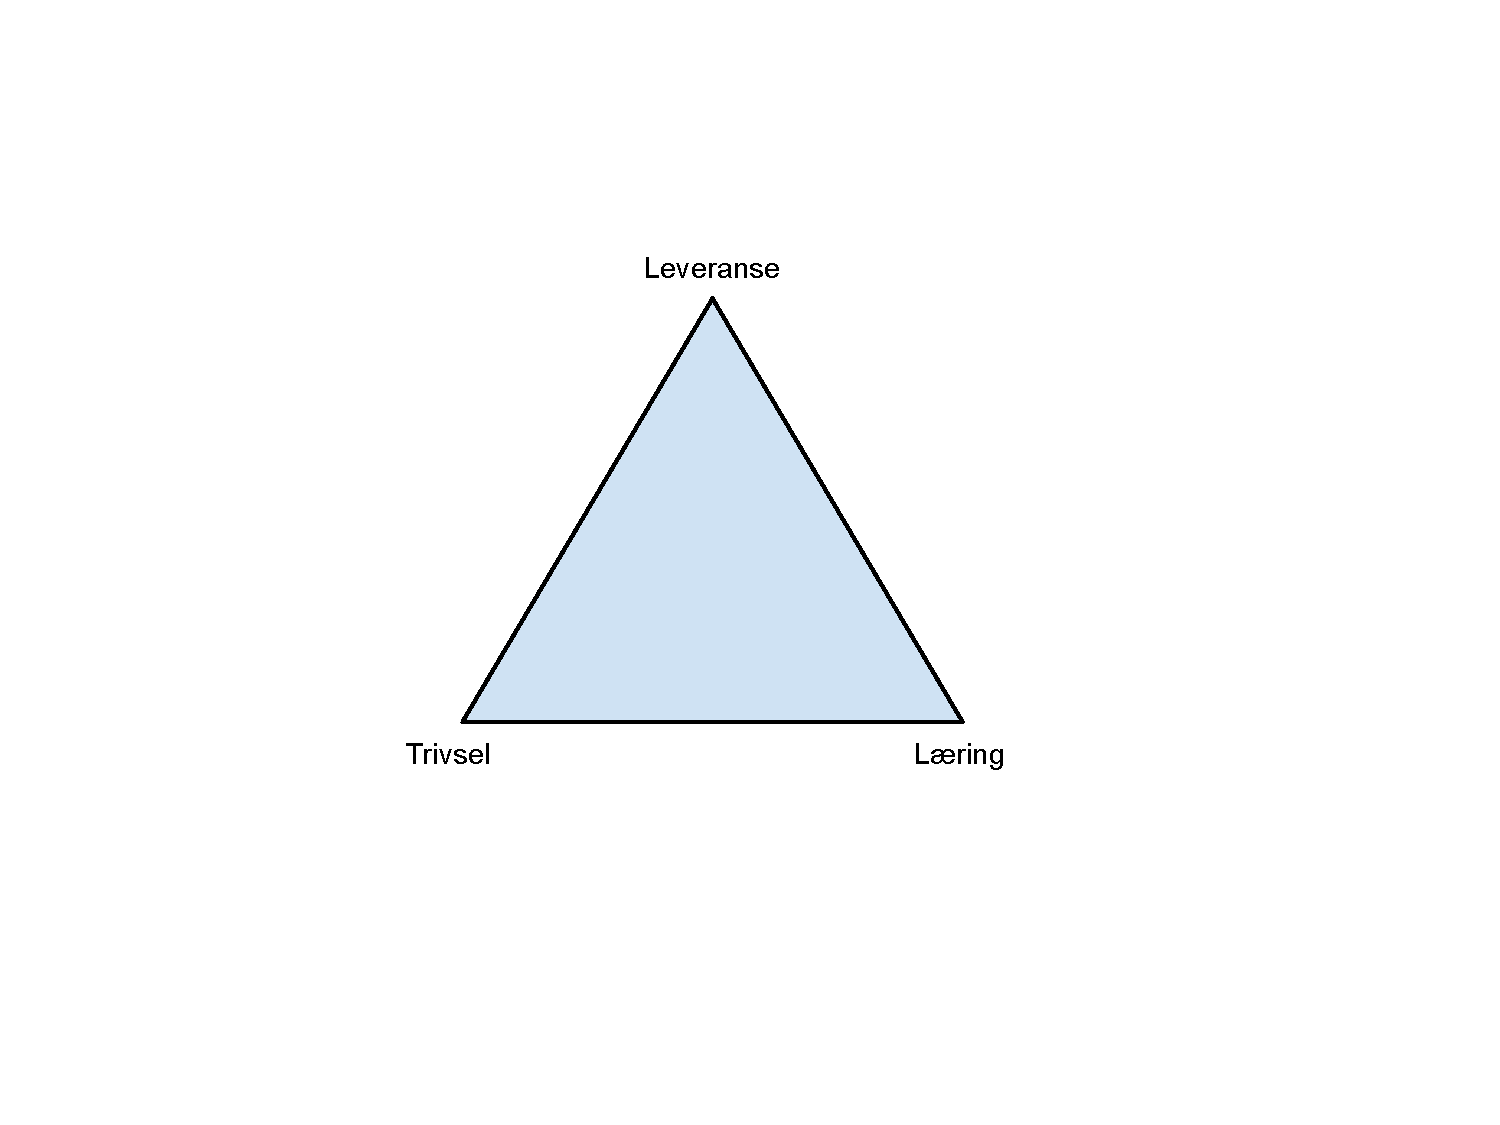
\includegraphics[clip=true, width=1 \textwidth,
trim=0cm 5cm 0cm 3cm]{kompetansetrekant.pdf}
\captionof{figure}{Kompetansetrekant}
\label{fig:kompetansetrekant}
\end{center}

Det ble i den grunn naturlig for oss å ta utgangspunkt i disse tre punktene når samarbeidsavtalen ble produsert. I punktet relatert til leveranse har vi fremhevet behovet for at de ulike gruppemedlemmene er bevisste på å ta ansvar for arbeid de utfører, og at dette arbeidet tilfredsstiller kravet om kvalitet som gruppa har blitt enig om. Et annet fokus innenfor leveranse har vært punktlighet og opprettholdelse av tidsfrister. Under trivsel har hovedfokuset blitt satt på inkludering. I tillegg har det vært viktig å være observante på eventuelle konflikter, og ta tak i disse på et tidlig tidspunkt før de eskalerer til et problem. Innenfor punktet læring har blikket blitt rettet mot deling av kunnskap. Det er viktig at medlemmene blir holdt oppdatert slik at alle kan bidra i diskusjoner. Videre er det poengtert i kontrakten at kritiske spørsmål må stilles slik at bevisstheten og kunnskapen økes.\\

\section{Samarbeidsverktøy}
Tidlig i prosjektet ble gruppa enig om hvilke verktøy som skulle benyttes for arbeid og kommunikasjon. Arbeidet var delt i to hovedgrupper: rapportskriving og programmering. Innenfor rapportskriving ble det naturlig å ta i bruk ``Google Docs" siden dette gav oss muligheten til å utføre simultant arbeid på både prosjekt- og prosessrapporten. Det førte også til at alle var oppdatert på progresjonen. Verktøyet var et viktig element i ønsket om å oppnå en høy effektivitet.\\

Innenfor programmering valgte vi i felleskap å ta i bruk ``git" som versjonskontroll. Begrunnelsen for valget var basert på at dette ville føre til en enkel måte å holde alle oppdatert på progresjonen samtidig som verktøyet er enkelt i bruk og gir backup hvis arbeid skulle gå tapt.\\

Som generell kommunikasjonskanal valgte vi å ta i bruk ``Facebook". Et slikt sosialt nettverk er godt egnet til den typen kommunikasjon som ble utført i løpet av prosjektet. Her kunne for eksempel medlemmer gi beskjed om de var forsinket til møtetider, eller gi andre beskjeder til resten av medlemmene når dette var nødvendig. Dette er i samsvar med punkt 2 i samarbeidsavtalen (\ref{appendix:samarbeidsavtale}): ``Alle møter til avtalt tid. Skjer det noe spesielt så skal det gis beskjed snarest mulig til hele gruppa på telefon eller Facebook om forsinkelser eller fravær. Ved mangel av beskjed blir dette tatt opp ved neste møte."\\
